\section{Ergebnisse}
Es werden Laufzeitmessungen durchgeführt, um die Auswirkung der Parallelisierung zu erfassen. Zur Vergleichbarkeit und Minimierung von Einflüssen durch sich ändernde Lasten der virtuellen Maschinen in der Cloud werden alle Messungen sequentiell vorgenommen. Zur Aufwandsbegrenzung wird eine Stichprobengröße von $n = 10$ Messungen pro Messklasse gewählt. Für eine statistisch fundierte Aussage notwendig wäre ein größere Anzahl an Messungen. Die Messklassen werden über die Anzahl der verwendeten Rechenknoten festgelegt. Messungen werden mit einem bis sieben Rechenknoten durchgeführt. Gemessen wird die benötigte Laufzeit, eine gleichbleibende Datei bestehend aus einer Zahl der Größenordnung von $400.000$ Wörtern zu sortieren. Mit einer Datei von doppelter Wörterzahl wird eine zweite Messreihe angefertigt.
\\
Eine Messergebnis ist die mithilfe der Standard Template Bibliothek std::chrono gemessene Zeit, welche im Programmablauf des Master-Knotens zwischen dem Zeitpunkt unmittelbar vor der Verteilung der Teilelemente 
des zu sortierenden Textes an die Slave-Knoten und dem Zeitpunkt unmittelbar nach dem Zusammenführen der Ergebnisse der Slave-Rechenknoten verstreicht.
Das arithmetische Mittel sowie die Standardabweichung der Messungen mit kürzerer Wörterzahl sind in der oberen Hälfte von Tabelle \ref{zeiten_tabelle_lang_und_kurz} aufgeführt. Die entsprechenden Werte zur größeren Datei sind in der unteren Hälfte von Tabelle \ref{zeiten_tabelle_lang_und_kurz} dargestellt.
\\
Bei der Messung mit kleiner Datei und genau einem Rechenknoten ist eine im Vergleich zu anderen Rechenknotenanzahlen erhöhte Unsicherheit zu erkennen. Die mittlere benötigte Rechenzeit ist signifikant höher als bei anderen Messungen mit einer Rechenknotenanzahl größer eins. Bei den Rechenknotenanzahlen vier, fünf und sechs ist eine im Vergleich geringe Abweichung festzustellen.
\\
Die Mittelwerte der Zeiten für die kleinere Datei liegen ab einer Rechenknotenanzahl von 4 eng beieinander. Mit den vorliegenden Daten kann keine statistisch begründete Aussage getroffen werden, ob sich die Rechenzeit ab einer Knotenzahl von 4 noch messbar verändert. Der scheinbar deutlich niedrigere Mittelwert der 7. Messung wird durch eine höhere Messunsicherheit relativiert.
\\
Dies kann auch im Kastenschaubild (Whisker Plot) zu den Messungen der kleineren Datei, Abbildung \ref{boxplot_times}, nachvollzogen werden. Ebenfalls ist eine deutliche 
der Laufzeiten über die Anzahl der Rechenknoten zu erkennen. Ebenfalls ist ein starker Ausreißer bei der Knotenzahl eins zu erkennen. Bei Knotenzahlen zwei, vier und sechs gibt es ebenfalls Ausreißer. Im Kontext der niedrigen Standardabweichung der Messungen mit Knotenzahlen vier und 6 bedeutet das einerseits, dass die weiteren Messwerte dieser Messung besonders konsistent sind. Andererseits kann dies ein Hinweis darauf sein, dass die gemessenen Zeiten durch Zufall besonders konsistent und niedrig ausgefallen sind.
\\
Die Ergebnisse der Messungen mit der größeren Datei sind in Abbildung \ref{boxplot_times_long} in Form eines Kastenschaubilds dargestellt. Im Vergleich zur kleineren Dateigröße sind hier weniger Ausreißer vorhanden und die absoluten Rechenzeiten sind durchweg höher.
\\
Bei beiden Dateigrößen ist mit steigender Rechenknotenzahl ein zunächst signifikanter Abfall der Rechenzeiten zu beobachten, bevor ein Effekt der Abflachung auftritt. Ab einer Rechenknotenzahl von vier bei der kleineren und fünf bei der größeren Datei kann kein weiterer signifikanter Abfall der Rechenzeit festgestellt werden.
\\
Beträgt die Laufzeit bei der kleineren Datei bei Knotenzahl eins ungefähr $4\text{s}$, so werden bei doppelter Wörteranzahl etwa $13\text{s}$ benötigt. Bei größeren Knotenzahlen beträgt die Rechenzeit für die kleine Datei etwa $1.7\text{s}$ und für die größere Datei ca. $5\text{s}$. Die beobachtete Absenkung der Laufzeit bewegt sich demnach in einer Größenordnung zwischen 50\% und 60\%.


\begin{table*}
	\caption{Zeitmessungen mit kleiner und großer Wörterzahl}
	\label{zeiten_tabelle_lang_und_kurz}
	\begin{tabularx}{\textwidth}{@{}l*{10}{C}c@{}}
		\toprule
		Anzahl der Rechenknoten & 1 & 2 & 3 & 4 & 5 & 6 & 7 \\ 
		\midrule
		$\bar{t}_{wenige Wörter}$ $\text{[ms]}$ & 4382.9 & 2413.7 & 2148.5 & 1728.6 & 1715.9 & 1621.6 & 1574.6 \\
		$\sigma_{wenige Wörter}$ $\text{[ms]}$ & 491.2 & 128.0 & 113.9 & 72.2 & 70.9 & 62.3 & 112.4 \\
		\addlinespace
		$\bar{t}_{viele Wörter}$ $\text{[ms]}$ & 13114.2 & 8857.0 & 6643.7 & 5913.3 & 5072.5 & 4727.8 & 4855.2 \\
		$\sigma_{viele Wörter}$ $\text{[ms]}$ & 99.3 & 240.1 & 202.2 & 261.0 & 125.1 & 105.0 & 180.1 \\
		\bottomrule
	\end{tabularx}
\end{table*}


\begin{figure}[!t]
	\centering
	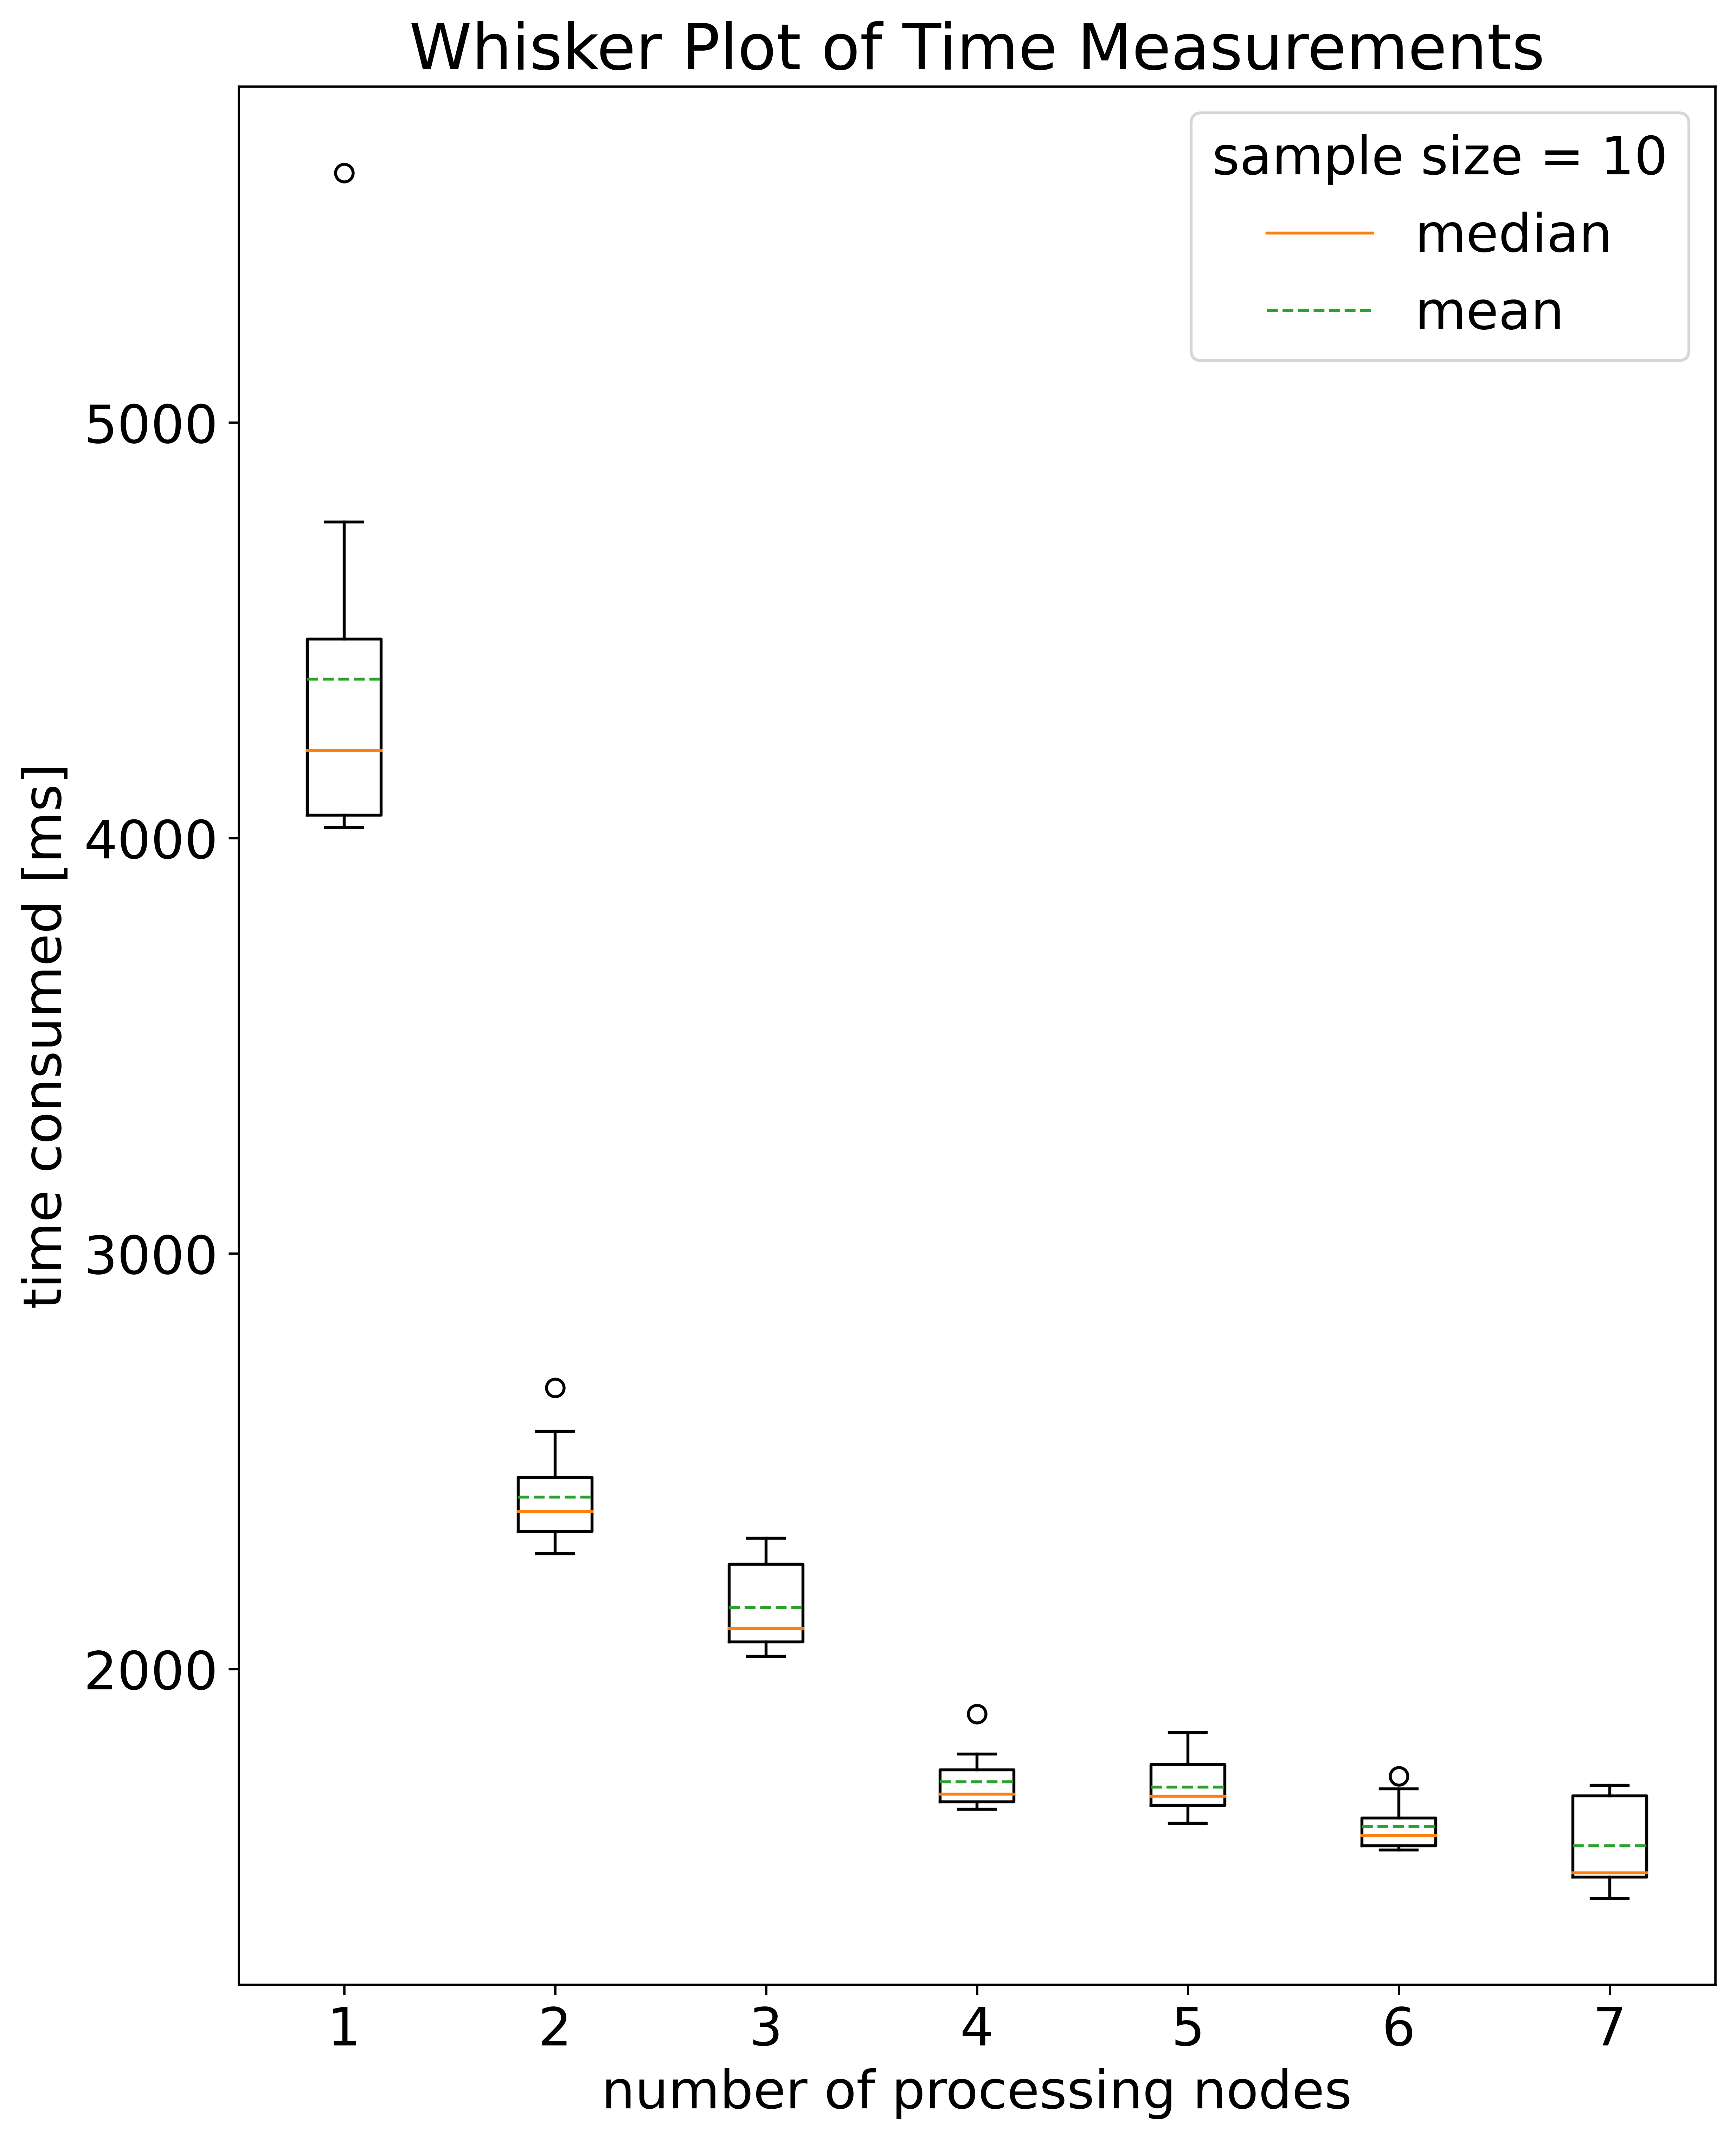
\includegraphics[width=3.5in]{boxplots.png}
	\caption{Messwerte zur kleineren der beiden getesteten Dateien dargestellt in einem Kastenschaubild}
	\label{boxplot_times}
\end{figure}
\begin{figure}[!t]
	\centering
	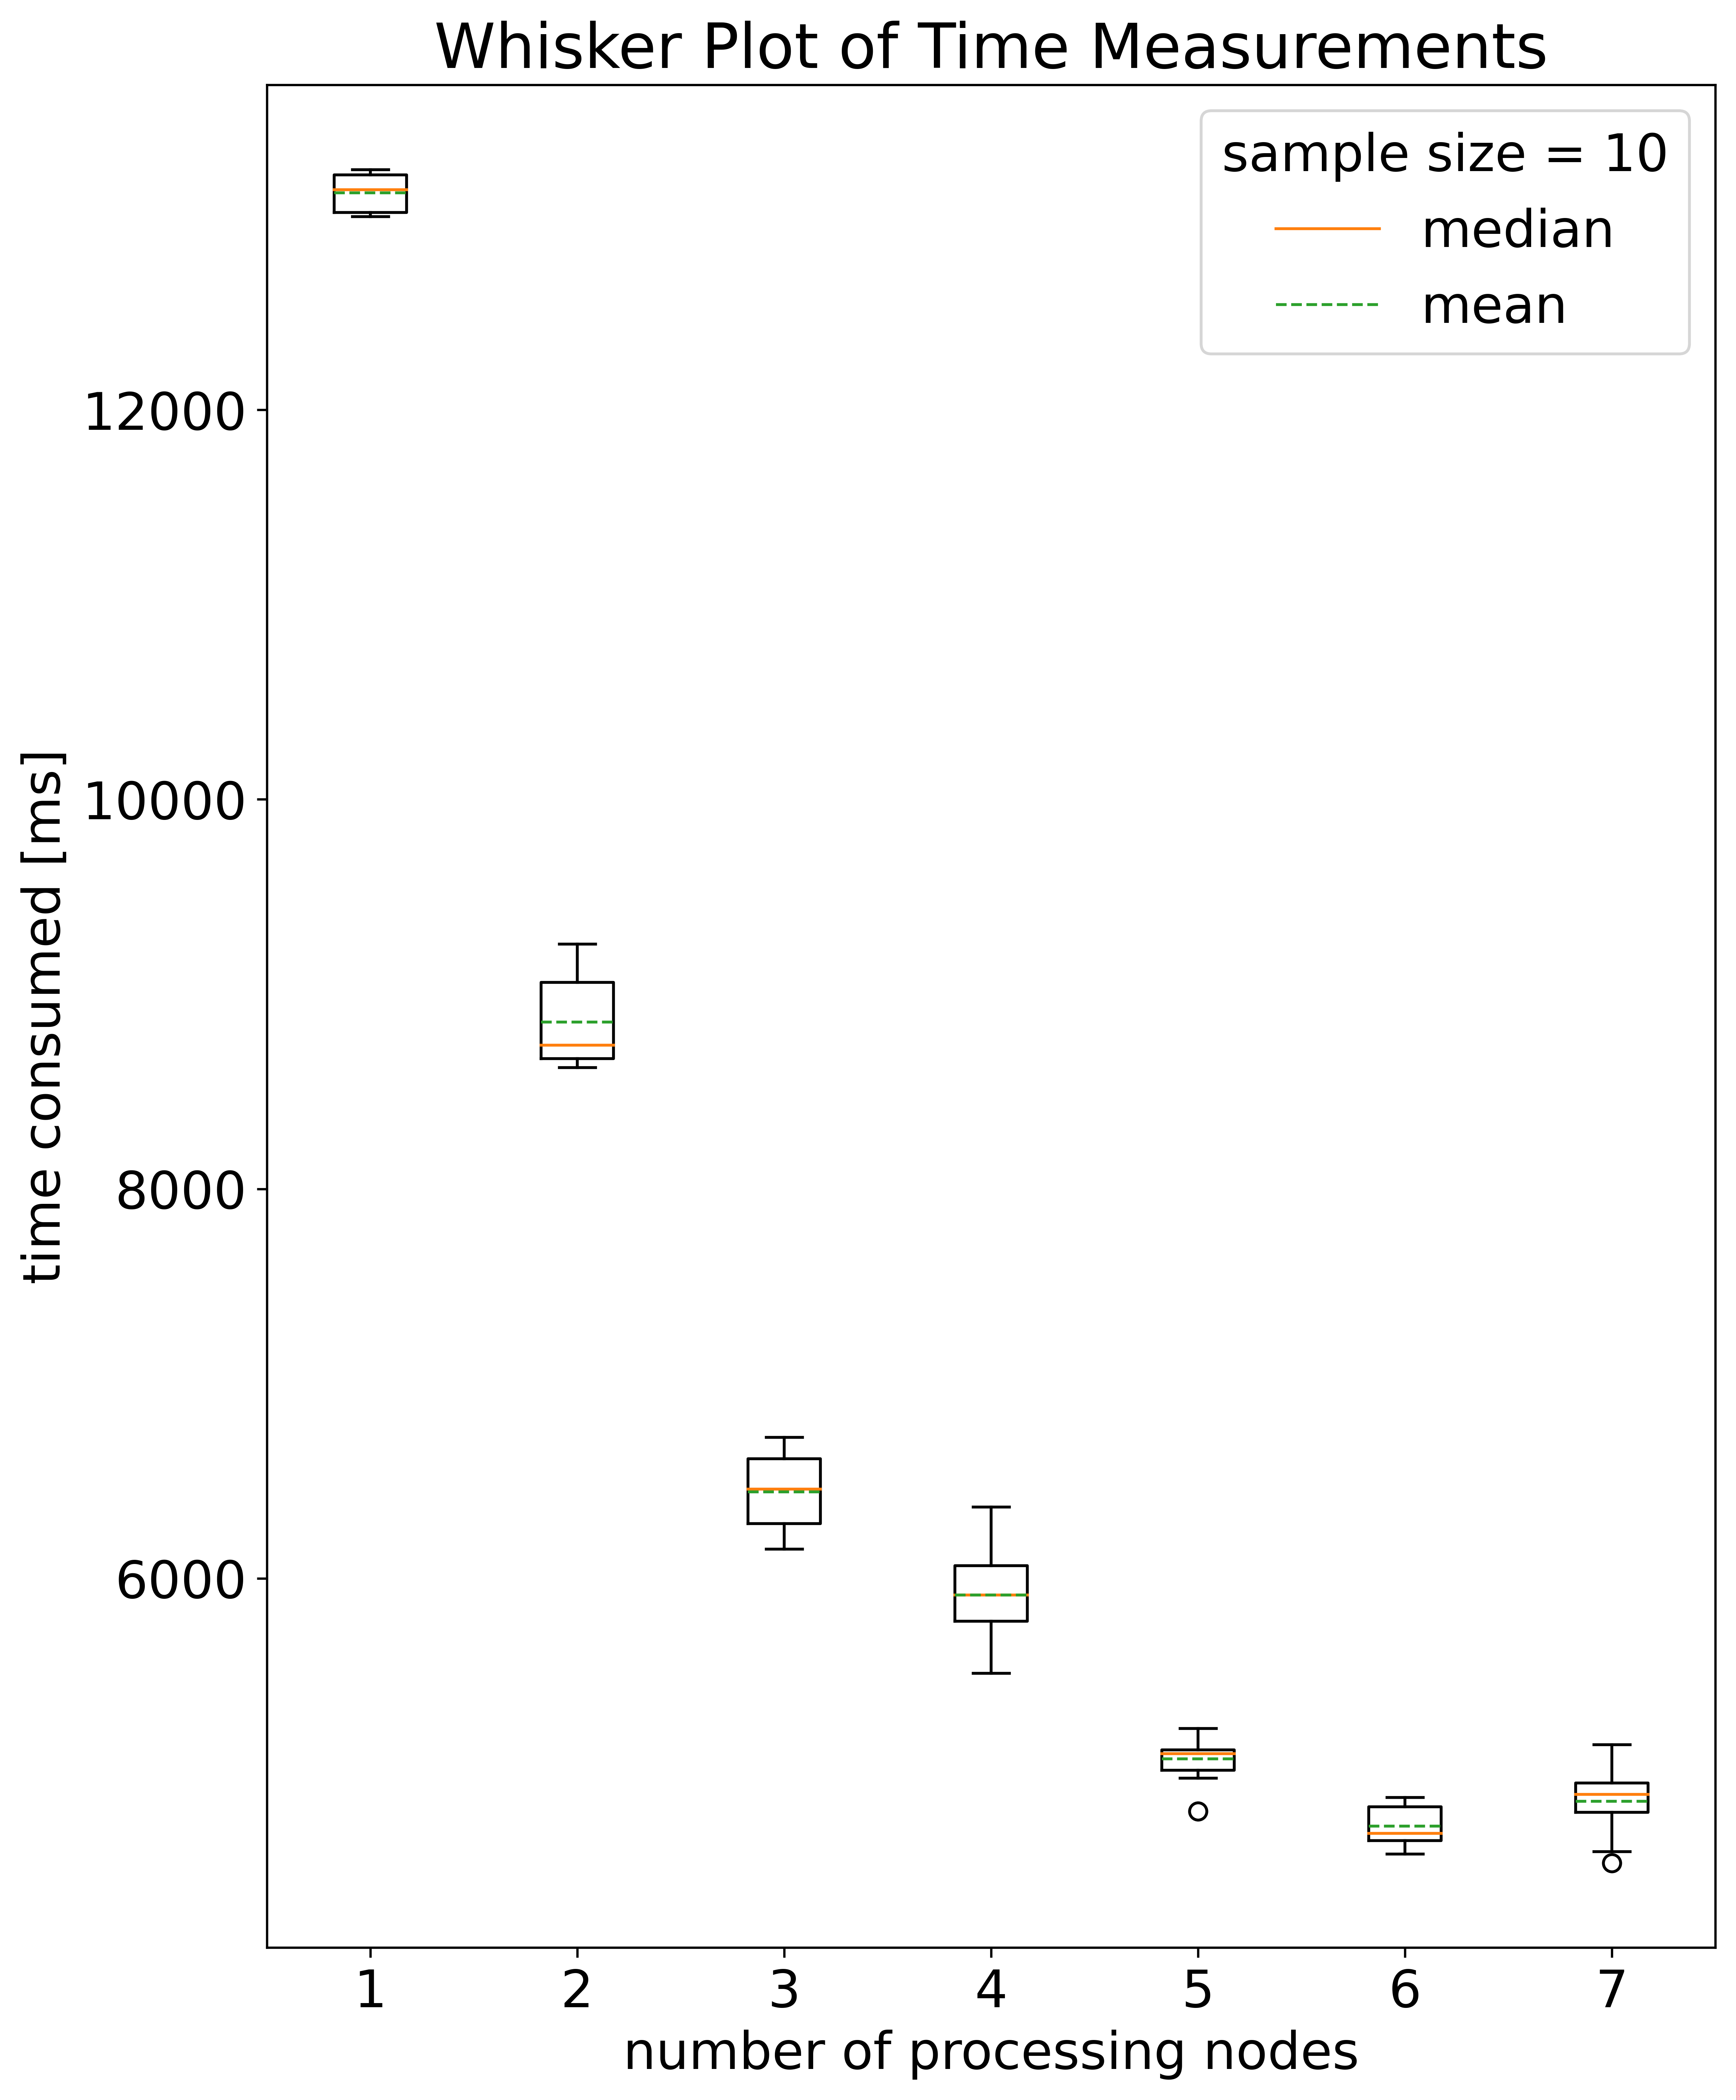
\includegraphics[width=3.5in]{boxplots_long.png}
	\caption{Messwerte zur größeren der beiden getesteten Dateien dargestellt in einem Kastenschaubild}
	\label{boxplot_times_long}
\end{figure}